\chapter{Von Shapley-Werten zu SHAP: Brückenschlag zur Modellinterpretation}

Im Rahmen der kooperativen Spieltheorie ermöglichen die Shapley-Werte eine faire Verteilung des kollektiv 
erwirtschafteten Nutzens auf die beteiligten Akteure. Diese Methodik findet eine analoge Anwendung 
in der Welt des maschinellen Lernens, um die Beiträge einzelner Merkmale zur Vorhersageleistung 
eines Modells zu bewerten \cite[S. 26]{Molnar_2023}. Hier wird die Terminologie der Shapley-Werte in den Kontext von Machine Learning 
Modellen übertragen, wobei jedes Merkmal als \glqq{}Spieler\grqq{} betrachtet wird, dessen Beitrag zur 
\glqq{}Auszahlung\grqq{} – der Vorhersage des Modells – evaluiert werden soll. 

\begin{table}[!h]
    \caption{Terminologie der originären Shapley-Werte im Kontext des maschinellen Lernens.}
    \footnotesize
    \begin{tabularx}{\textwidth}{XXX}
    \toprule
    Terminologie Konzept & Terminologie Machine Learning & Ausdruck \\
    \midrule
    Spieler & Merkmal Index & $j$ \\
    Anzahl aller Spieler & Anzahl aller Merkmale & $p$ \\
    Große Koalition & Menge aller Merkmale & $\mathcal{N} = \{1, \ldots, p\}$\\
    Koalition & Menge von Merkmalen & $\mathcal{S} \subseteq \mathcal{N}$ \\
    Größe der Koalition & Anzahl der Merkmale in der Koalition $\mathcal{S}$ & $|\mathcal{S}|$\\
    Spieler, die nicht in der Koalition sind & Merkmale, die nicht in der Koalition enthalten sind & $C: C = \mathcal{N} \setminus \mathcal{S}$ \\
    Koalitionsfunktion & Vorhersage für Merkmalswerte in der Koalition $\mathcal{S}$ abzüglich der Vorhersage im Mittel & $v_{f, x^{(i)}}(\mathcal{S}$)\\
    Auszahlung & Vorhersage für eine Beobachtung $x^{(i)}$ abzüglich der Vorhersage im Mittel & $f(x^{(i)}) -  \mathbb{E}(f(X))$\\
    Shapley-Wert & Beitrag des Merkmals $j$ zur Auszahlung des Modells für eine Beobachtung $x^{(i)}$& $\varphi_j^{(i)}(\mathcal{N}, f)$\\
    \bottomrule
    \end{tabularx}
    \label{tab:shapley_terms}
    \normalsize\\
    Quelle: \cite[S. 26]{Molnar_2023}.
\end{table}

Die Koalitionsfunktion $v_{f, x^{(i)}}(\mathcal{S})$ für ein gegebenes Model $f$ und eine Beobachtung $x^{(i)}$ ist definiert als:

\begin{align}
    \label{eq:shap-value-func}
    v_{f, x^{(i)}}(\mathcal{S}) = \int_{\mathbb{R}} f(x^{(i)}_{\mathcal{S}} \cup X_{C}) d\mathbb{P}_{X_{C}} - \mathbb{E}(f(X))
\end{align}

Diese Funktion berechnet den erwarteten Wert der Vorhersage des Modells $f$, wenn nur eine Teilmenge $\mathcal{S}$ der 
Merkmale genutzt wird, um die Vorhersage für die spezifische Beobachtung $x^{(i)} \in \mathbb{R}^{p}$ zu treffen. 
Das Integral $\int_{\mathbb{R}}$ repräsentiert die Berechnung dieses erwarteten Wertes über alle möglichen Werte der Merkmale, 
die nicht in $\mathcal{S}$ enthalten sind ($X_C$), gewichtet durch deren Wahrscheinlichkeitsverteilung $\mathbb{P}_{X_{C}}$. 
Die Differenz zum Erwartungswert der Vorhersagen über alle Merkmale $\mathbb{E}(f(X))$ zeigt, 
wie viel die spezifische Menge an Merkmalen $\mathcal{S}$ zur Vorhersage beiträgt \cite[S. 221, S. 27]{Molnar_2022, Molnar_2023}.

Der marginale Beitrag eines Merkmals $j$ zu einer Koalition $\mathcal{S}$ ist dann:

\begin{align}
    \label{eq:shap-marginal-func}
    v_{f, x^{(i)}}(\mathcal{S} \cup \{j\}) - v_{f, x^{(i)}}(\mathcal{S}) &= \int_{\mathbb{R}} f(x^{(i)}_{\mathcal{S} \cup \{j\}} \cup X_{C \setminus \{j\}}) d\mathbb{P}_{X_{C \setminus \{j\}}} - \mathbb{E}(f(X)) \\ \notag
    &\quad - \left( \int_{\mathbb{R}} f(x^{(i)}_{\mathcal{S}} \cup X_{C}) d\mathbb{P}_{X_{C}} - \mathbb{E}(f(X)) \right) \\ \notag
    &= \int_{\mathbb{R}} f(x^{(i)}_{\mathcal{S} \cup \{j\}} \cup X_{C \setminus \{j\}}) d\mathbb{P}_{X_{C \setminus \{j\}}} \\ \notag
    &\quad - \int_{\mathbb{R}} f(x^{(i)}_{\mathcal{S}} \cup X_{C}) d\mathbb{P}_{X_{C}}
\end{align}

Diese Gleichung beschreibt, wie sich der erwartete Wert der Vorhersage ändert, wenn das Merkmal $j$ zu der Menge der Merkmale $\mathcal{S}$ hinzugefügt wird \cite[S. 29]{Molnar_2023}.

Der Beitrag $\varphi_j^{(i)}(\mathcal{N}, f)$ eines Merkmals $j$ für eine Beobachtung $x^{(i)} \in \mathbb{R}^{p}$ für die Vorhersage $f(x^{(i)})$ ist gegeben als:

\begin{align}
    \label{eq:shap-eq}
    \varphi^{(i)}_{j} (\mathcal{N}, f) &= \sum_{\mathcal{S} \subseteq \mathcal{N} \setminus \{j\}} \frac{|\mathcal{S}|! \cdot (p - 1 - |\mathcal{S}|)!}{p!} \\ \notag
    &\quad \cdot \left( \int_{\mathbb{R}} f(x^{(i)}_{\mathcal{S} \cup \{j\}} \cup X_{C \setminus \{j\}}) d\mathbb{P}_{X_{C \setminus \{j\}}} -
    \int_{\mathbb{R}} f(x^{(i)}_{\mathcal{S}} \cup X_{C}) d\mathbb{P}_{X_{C}} \right) 
\end{align}

Diese Formel ist die zentrale Berechnung der SHAP-Werte im maschinellen Lernen. 
Sie summiert den gewichteten, marginalen Beitrag des Merkmals $j$ über alle möglichen Kombinationen der anderen Merkmale. 
Die Gewichtung berücksichtigt die Anzahl der Merkmale in der Koalition $\mathcal{S}$ und die Anzahl der verbleibenden Merkmale, 
die noch hinzugefügt werden können. Dies ergibt den durchschnittlichen Beitrag des Merkmals $j$ zur Vorhersage für die 
Beobachtung $x^{(i)}$ \cite[S. 29, 30]{Molnar_2023}.

Die Integration in der SHAP-Formel ist ein zentraler Schritt, um den erwarteten Beitrag jedes Merkmals unter 
Berücksichtigung der gesamten Verteilung der Daten zu ermitteln. 
In diesem Ansatz werden die Merkmale als Zufallsvariablen behandelt, und die Integration erfolgt über 
die Wahrscheinlichkeitsverteilungen dieser Zufallsvariablen. Durch das Berechnen der erwarteten Vorhersagewerte mit 
und ohne des jeweiligen Merkmals, unter Einbeziehung der Verteilung aller anderen Merkmale, 
ermöglicht SHAP eine präzise und umfassende Einschätzung des Einflusses jedes einzelnen Merkmals. 
Dieser Prozess der Marginalisierung, bei dem man über die Wahrscheinlichkeitsverteilungen der Merkmale integriert, 
erlaubt es, den Beitrag eines jeden Merkmals zu isolieren und unabhängig von der spezifischen Zusammensetzung 
der anderen Merkmale zu bewerten. Dies führt zu einer fairen und ganzheitlichen Bewertung der Beiträge aller Merkmale 
zur Vorhersage des Modells \cite[S. 28]{Molnar_2023}.

\section{Berechnung der SHAP-Werte unter Berücksichtigung der zugrundeliegenden Verteilung}
\label{sec:example}

Ein einfaches Beispiel soll helfen, die Anwendung von SHAP-Werten im 
Kontext des maschinellen Lernens zu illustrieren\footnote{In Anlehnung an das Beispiel aus Kapitel 8.5.1 \glqq{}General Idea\grqq{} \cite[S.215f]{Molnar_2022}.}. Betrachtet wird ein fiktiver 
Immobilien-Datensatz mit drei Merkmalen: Größe des Hauses in Quadratmetern ($x_1$), Anzahl der Zimmer ($x_2$) 
und Entfernung zum Stadtzentrum in Kilometern ($x_3$). Es gibt zwei Beobachtungen in diesem Datensatz:

\begin{table}[!h]
    \caption{Merkmale von Beobachtungen in einem Immobilien-Datensatz.}
    \footnotesize
    \begin{tabularx}{\textwidth}{Xrrr}
    \toprule
     & $x_1$: Größe (in $m^2$) &  $x_2$: Anzahl Zimmer &  $x_3$: Entfernung zum Zentrum (in km) \\
    \midrule
    $x^{(1)}$ & 100 & 3 & 5 \\
    $x^{(2)}$ & 150 & 4 & 10 \\
    \bottomrule
    \end{tabularx}
    \label{tab:example}
    \normalsize\\
    Quelle: Eigene Darstellung.
\end{table}

Angenommen das Modell $f(x^{(i)})$ prognostiziert den Preis eines Hauses in Euro als eine lineare Kombination der Merkmale:

\begin{equation}
    f(x^{(i)}) = 5x_1^{(i)} + 20x_2^{(i)} - 2x_3^{(i)}.
\end{equation}

Die Vorhersagen für die beiden Beobachtungen lauten dann:

\begin{align}
    \label{eq:fx1}
    f(x^{(1)}) &= 5x_1^{(1)} + 20x_2^{(1)} - 2x_3^{(1)} \\ \notag
        &= 5 \cdot 100 + 20 \cdot 3 - 2 \cdot 5 \\ \notag
        &= 550\,\text{\euro} 
\end{align}

und 

\begin{align}
    f(x^{(2)}) &= 5x_1^{(2)} + 20x_2^{(2)} - 2x_3^{(2)} \\ \notag
        &= 5 \cdot 150 + 20 \cdot 4 - 2 \cdot 10 \\ \notag
        &= 810\,\text{\euro}. 
\end{align}

Die erwartete Auszahlung des Modells $\mathbb{E}(f(X))$ wird berechnet als:
\begin{align}
    \label{eq:efx}
    \mathbb{E}(f(X)) &= 5 \cdot \mathbb{E}(X_1) + 20 \cdot \mathbb{E}(X_2) - 2 \cdot \mathbb{E}(X_3) \\ \notag
                     &= 5 \cdot 125 + 20 \cdot 3,5 - 2 \cdot 7,5 \\ \notag
                     &= 680 \,\text{\euro},
\end{align}

mit 

\begin{align}
    \label{eq:e}
    \mathbb{E}(X_j) = \frac{1}{n} \sum_{i=1}^{n} x_j^{(i)}.
\end{align}     

Sei $\mathcal{N} = \{1, 2, 3\}$ die Menge aller Merkmale und die Beobachtung $x^{(1)} = [100, 3, 5]$. 
Der SHAP-Wert für jedes Merkmal $j \in \mathcal{N}$ wird unter Berücksichtigung der Verteilung der 
Daten und der Formel \ref{eq:shap-eq} berechnet:

\begin{align}
    \label{eq:shap-formular}
    \varphi^{(1)}_{j} (\mathcal{N}, f) &= \sum_{\mathcal{S} \subseteq \mathcal{N} \setminus \{j\}} \frac{|\mathcal{S}|! \cdot (p - 1 - |\mathcal{S}|)!}{p!} \\ \notag
    &\quad \cdot \left( \int_{\mathbb{R}} f(x^{(1)}_{\mathcal{S} \cup \{j\}} \cup X_{C \setminus \{j\}}) d\mathbb{P}_{X_{C \setminus \{j\}}} -
    \int_{\mathbb{R}} f(x^{(1)}_{\mathcal{S}} \cup X_{C}) d\mathbb{P}_{X_{C}} \right) 
\end{align}

wobei $p = |\mathcal{N}| = 3$ die Anzahl der Merkmale ist und $X_C$ die Menge der Merkmale 
außerhalb der Koalition $\mathcal{S}$ repräsentiert. Die Integrale repräsentieren die erwartete 
Vorhersage des Modells über die Verteilung der nicht in der Koalition enthaltenen Merkmale.

In linearen Modellen, unter der Prämisse, dass die Merkmale unabhängig voneinander und identisch verteilt sind, 
ist es möglich, die Berechnung der SHAP-Werte zu vereinfachen. Anstelle der komplexen Integration 
über die Verteilungen aller Merkmale, kann der Fokus auf die Unterschiede in den Modellvorhersagen gelegt werden, 
die sich aus dem Hinzufügen oder Entfernen einzelner Merkmale ergeben. 
Hierbei wird anstelle der spezifischen Werte der nicht in der betrachteten Koalition enthaltenen Merkmale 
die Erwartungswerte herangezogen. Diese Vereinfachung ermöglicht es, den Einfluss jedes Merkmals auf 
die Modellvorhersage auf eine direktere und rechnerisch weniger aufwendige Weise zu erfassen.
Diese Vereinfachung ist für lineare Modelle angemessen, da die Auswirkungen jedes Merkmals 
auf die Vorhersage des Modells additiv und unabhängig sind \cite[S. 48]{Molnar_2023}. Bei komplexeren, 
nichtlinearen Modellen ist eine detailliertere Berechnung erforderlich, 
die oft auf numerischen Methoden oder Annäherungen basiert, mehr dazu in Kapitel \ref{sec:estimators}.

Der Beitrag durch das Hinzufügen des Merkmals $x_1$ zur bestehenden Koalition $\mathcal{S} = \{x_2\}$ wird
nach Formel \ref{eq:shap-formular} berechnet als:

\begin{align}
    \varphi^{(1)}_{1}(\{x_2\}, f) &= \frac{1! \cdot (3 - 1 - 1)!}{3!} \\ \notag
        &\quad \cdot \int f(x_1, x_2 , X_3) d\mathbb{P}(X_3) - \int f(X_1, x_2, X_3) d\mathbb{P}(X_1, X_3)
\end{align}

Da \( X_1 \) und \( X_3 \) unabhängig und identisch verteilt sind, können \( X_2 \) und \( X_3 \) durch ihre Erwartungswerte (Gleichung \ref{eq:e}) ersetzt werden:

\begin{align}
    \varphi^{(1)}_{1}(\{x_2\}, f) &= \frac{1}{6} \Big(f(x_1, x_2, \mathbb{E}(X_3)) - f(\mathbb{E}(X_1), x_2, \mathbb{E}(X_3))\Big) \\ \notag
        &= \frac{1}{6} \Big( f(100, 3, 7.5) - f(125, 3, 7.5) \Big) \\ \notag
        &= \frac{1}{6} \Big( (5 \cdot 100 + 20 \cdot 3 - 2 \cdot 7,5) - (5 \cdot 125 + 20 \cdot 3 - 2 \cdot 7,5) \Big) \\ \notag
        &= \frac{1}{6} (545 - 670) \\ \notag
        &= \frac{1}{6} (-125)
\end{align}
 
Die in Tabelle \ref{tab:shapley_marginal_features_x1} dargestellten Kombinationen illustrieren die marginalen Beiträge und SHAP-Werte 
für jedes Merkmal in jeder möglichen Koalition von Merkmalen, bezogen auf die Beobachtung $x^{(1)}$. 

\begin{table}[!h]
    \caption{Marginalbeiträge der einzelnen Merkmale zu den möglichen Koalitionen für die Beobachtung $x^{(1)}$.}
    \footnotesize
    \begin{tabularx}{\textwidth}{XXrrrrr}
    \toprule
    $x_{j}$ & $\mathcal{S}$ & $v_{f, x^{(1)}}(\mathcal{S})$ & $v_{f, x^{(1)}}(\mathcal{S} \cup \{j\})$ & $v_{f, x^{(1)}}(\mathcal{S} \cup \{j\}) - v_{f, x^{(1)}}(\mathcal{S})$ & Gewicht & $\varphi_{j}^{(1)}(\mathcal{S}, f)$\\
    \midrule
    $x_1$ & $\emptyset$ & 680 & 555 & -125 & $\frac{1}{3}$ & -41,67 \\
    $x_1$ & $\{x_2\}$ & 670 & 545 & -125 & $\frac{1}{6}$ & -20.83 \\
    $x_1$ & $\{x_3\}$ & 685 & 560 & -125 & $\frac{1}{6}$ & -20.83 \\
    $x_1$ & $\{x_2, x_3\}$ & 675 & 550 & -125 & $\frac{1}{3}$ & -41,67 \\
    $x_2$ & $\emptyset$ & 680 & 670 & -10 & $\frac{1}{3}$ & -3,33 \\
    $x_2$ & $\{x_1\}$ & 555 & 545 & -10 & $\frac{1}{6}$ & -1,67 \\
    $x_2$ & $\{x_3\}$ & 685 & 675 & -10 & $\frac{1}{6}$ & -1,67 \\
    $x_2$ & $\{x_1, x_3\}$ & 560 & 550 & -10 & $\frac{1}{3}$ & -3,33 \\
    $x_3$ & $\emptyset$ & 680 & 685 & 5 & $\frac{1}{3}$ & 1,67 \\
    $x_3$ & $\{x_1\}$ & 555 & 560 & 5 & $\frac{1}{6}$ & 0,83 \\
    $x_3$ & $\{x_2\}$ & 670 & 675 & 5 & $\frac{1}{6}$ & 0,83 \\
    $x_3$ & $\{x_1, x_2\}$ & 545 & 550 & 5 & $\frac{1}{3}$ & 1,67 \\
    \bottomrule
    \end{tabularx}
    \label{tab:shapley_marginal_features_x1}
    \normalsize\\
    Quelle: Eigene Darstellung.
\end{table}

Diese Analyse ist ebenso auf die Beobachtung $x^{(2)}$ anwendbar und erfordert eine analoge Vorgehensweise, 
wie in Tabelle \ref{tab:shapley_marginal_features_x2} dargestellt:

\begin{table}[!h]
    \caption{Marginalbeiträge der einzelnen Merkmale zu den möglichen Koalitionen für die Beobachtung $x^{(2)}$.}
    \footnotesize
    \begin{tabularx}{\textwidth}{XXrrrrr}
    \toprule
    $x_{j}$ & $\mathcal{S}$ & $v_{f, x^{(2)}}(\mathcal{S})$ & $v_{f, x^{(2)}}(\mathcal{S} \cup \{j\})$ & $v_{f, x^{(2)}}(\mathcal{S} \cup \{j\}) - v_{f, x^{(2)}}(\mathcal{S})$ & Gewicht & $\varphi_{j}^{(2)}(\mathcal{S}, f)$\\
    \midrule
    $x_1$ & $\emptyset$ & 680 & 805 & 125 & $\frac{1}{3}$ & 41,67 \\
    $x_1$ & $\{x_2\}$ & 690 & 815 & 125 & $\frac{1}{6}$ & 20.83 \\
    $x_1$ & $\{x_3\}$ & 675 & 800 & 125 & $\frac{1}{6}$ & 20.83 \\
    $x_1$ & $\{x_2, x_3\}$ & 685 & 810 & 125 & $\frac{1}{3}$ & 41,67 \\
    $x_2$ & $\emptyset$ & 680 & 690 & 10 & $\frac{1}{3}$ & 3,33 \\
    $x_2$ & $\{x_1\}$ & 805 & 815 & 10 & $\frac{1}{6}$ & 1,67 \\
    $x_2$ & $\{x_3\}$ & 675 & 685 & 10 & $\frac{1}{6}$ & 1,67 \\
    $x_2$ & $\{x_1, x_3\}$ & 800 & 810 & 10 & $\frac{1}{3}$ & 3,33 \\
    $x_3$ & $\emptyset$ & 680 & 675 & -5 & $\frac{1}{3}$ & -1,67 \\
    $x_3$ & $\{x_1\}$ & 805 & 800 & -5 & $\frac{1}{6}$ & -0,83 \\
    $x_3$ & $\{x_2\}$ & 690 & 685 & -5 & $\frac{1}{6}$ & -0,83 \\
    $x_3$ & $\{x_1, x_2\}$ & 815 & 810 & -5 & $\frac{1}{3}$ & -1,67 \\
    \bottomrule
    \end{tabularx}
    \label{tab:shapley_marginal_features_x2}
    \normalsize\\
    Quelle: Eigene Darstellung.
\end{table}

Die in den Tabellen \ref{tab:shapley_marginal_features_x1} und \ref{tab:shapley_marginal_features_x2} 
dargestellten SHAP-Werte für die Beobachtungen \( x^{(1)} \) und \( x^{(2)} \) zeigen eine interessante Symmetrie. 
Für jedes Merkmal entspricht der SHAP-Wert für \( x^{(2)} \) genau dem negativen Wert für \( x^{(1)} \). 
Die beobachtete Inversion der SHAP-Werte zwischen den Beobachtungen \( x^{(1)} \) und \( x^{(2)} \) 
lässt sich durch die zentrale Rolle des Erwartungswerts des Modells erklären. 
Das Modell prognostiziert im Mittel einen Immobilienpreis von 680 \euro. In einem Szenario, in dem nur zwei 
Beobachtungen vorhanden sind, spiegeln die Beobachtungen \( x^{(1)} \) und \( x^{(2)} \) entgegengesetzte 
Abweichungen vom Erwartungswert wider. Die SHAP-Werte, die den Beitrag jedes Merkmals zur Abweichung 
der Vorhersage vom Mittelwert messen, zeigen daher für \( x^{(1)} \) und \( x^{(2)} \) genau entgegengesetzte Werte. 
Dieses Phänomen resultiert aus der Tatsache, dass die Merkmalsbeiträge in Bezug auf den Erwartungswert 
berechnet werden und unsere beispielhaften Beobachtungen symmetrisch um diesen Mittelwert verteilt sind. 
Folglich heben sich ihre Beiträge im Kontext unseres linearen Modells exakt auf, was die Konsistenz und 
Zuverlässigkeit der SHAP-Wert-Berechnung unterstreicht.


\begin{figure}[!h]
    \caption{Beitrag der Merkmale $x_{j \in \{1, 2, 3\}}$ zur Modellvorhersage $f(x^{(1)})$.}
    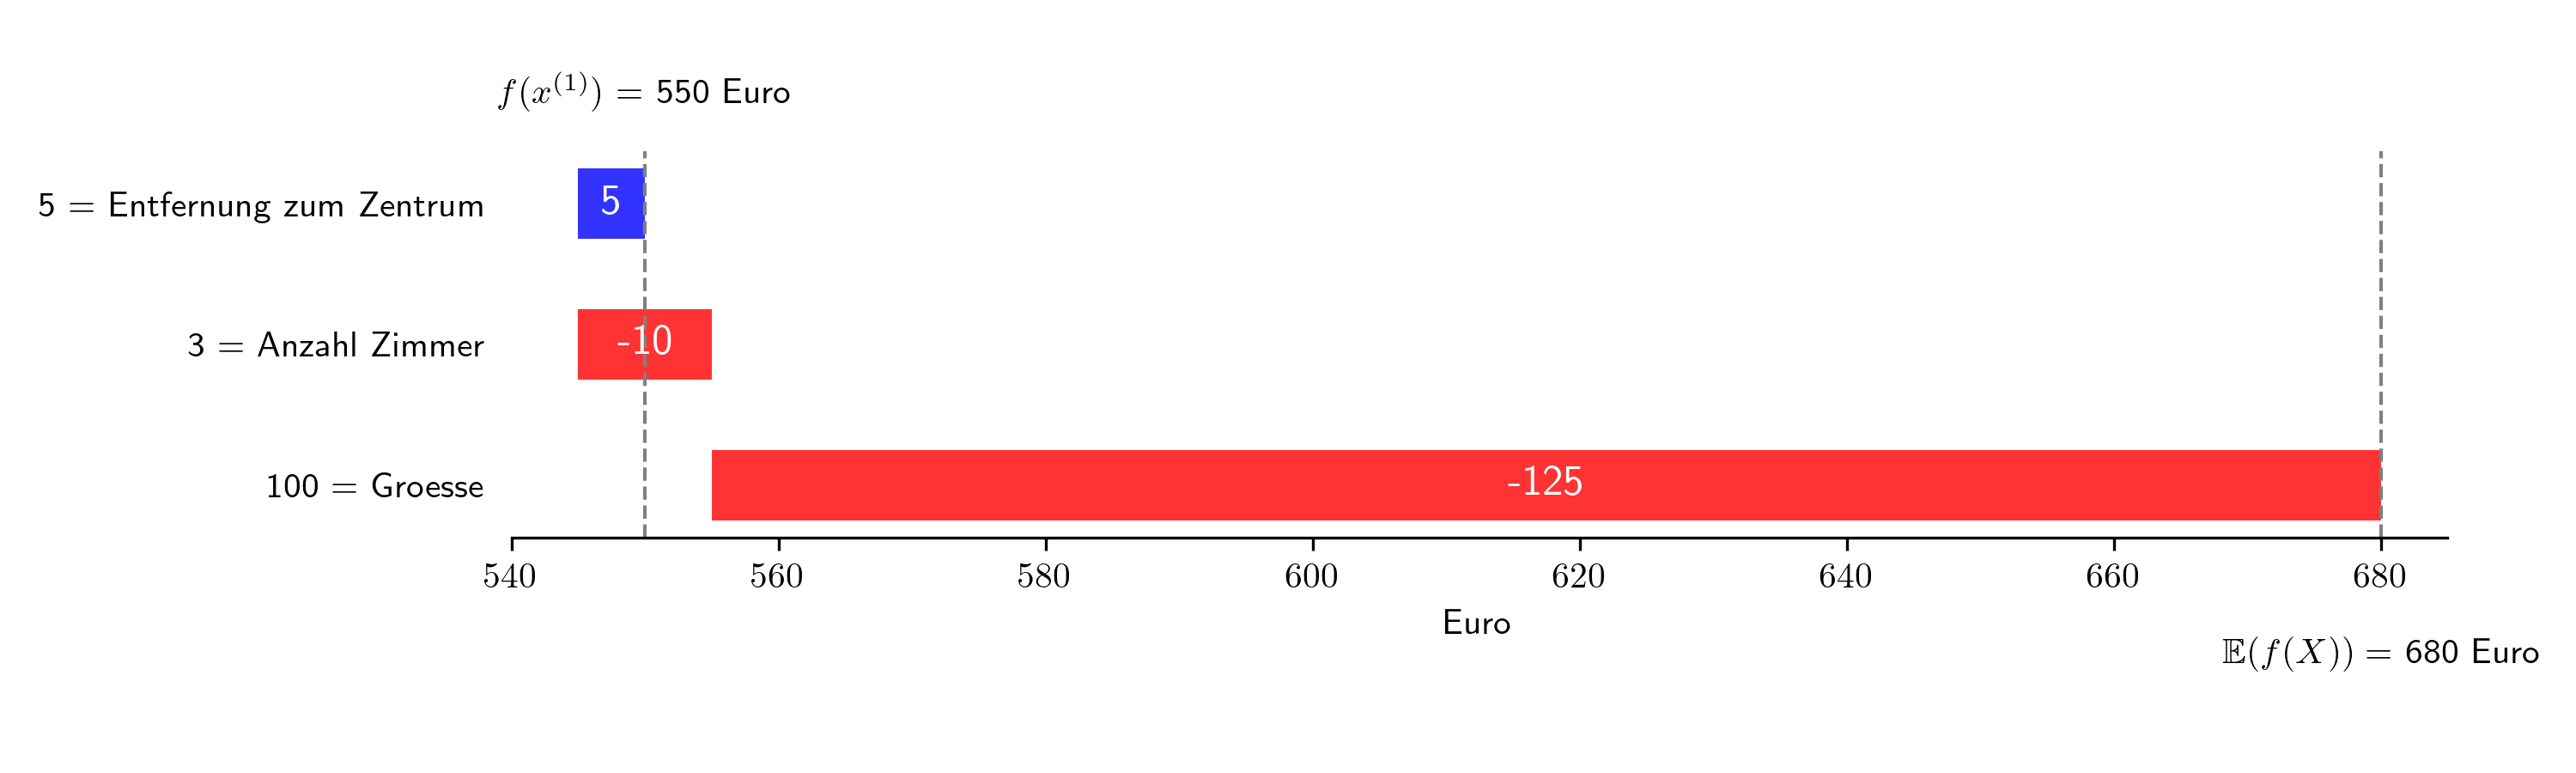
\includegraphics[width=1\textwidth]{../scripts/images/model-output-x1.png}
    Quelle: Eigene Darstellung, \ref{charts}.
    \label{pic:model-fx1}
\end{figure}

Das Modell $f(x^{(i)})$
prognostiziert im Mittel einen Immobilienpreis von 680 \euro{}. Im Vergleich zur
Verteilung des jeweiligen Merkmals, reduziert die Größe der 
Wohnung ($x_1^{(1)}$) und die Anzahl der Zimmer ($x_2^{(1)}$) die Prognose 
des Preises für die Immobilie $x^{(1)}$ um insgesamt 135 \euro{}, während die Entfernung zum Stadtzentrum
($x_3^{(1)}$) den Preis der Wohnung um 5 \euro{} erhöht, wie in Abbildung 
\ref{pic:model-fx1} veranschaulicht. Abbildung \ref{pic:model-fx2} visualisiert die SHAP-Werte für die Immobilie $x^{(2)}$:

\begin{figure}[!h]
    \caption{Beitrag der Merkmale $x_{j \in \{1, 2, 3\}}$ zur Modellvorhersage $f(x^{(2)})$.}
    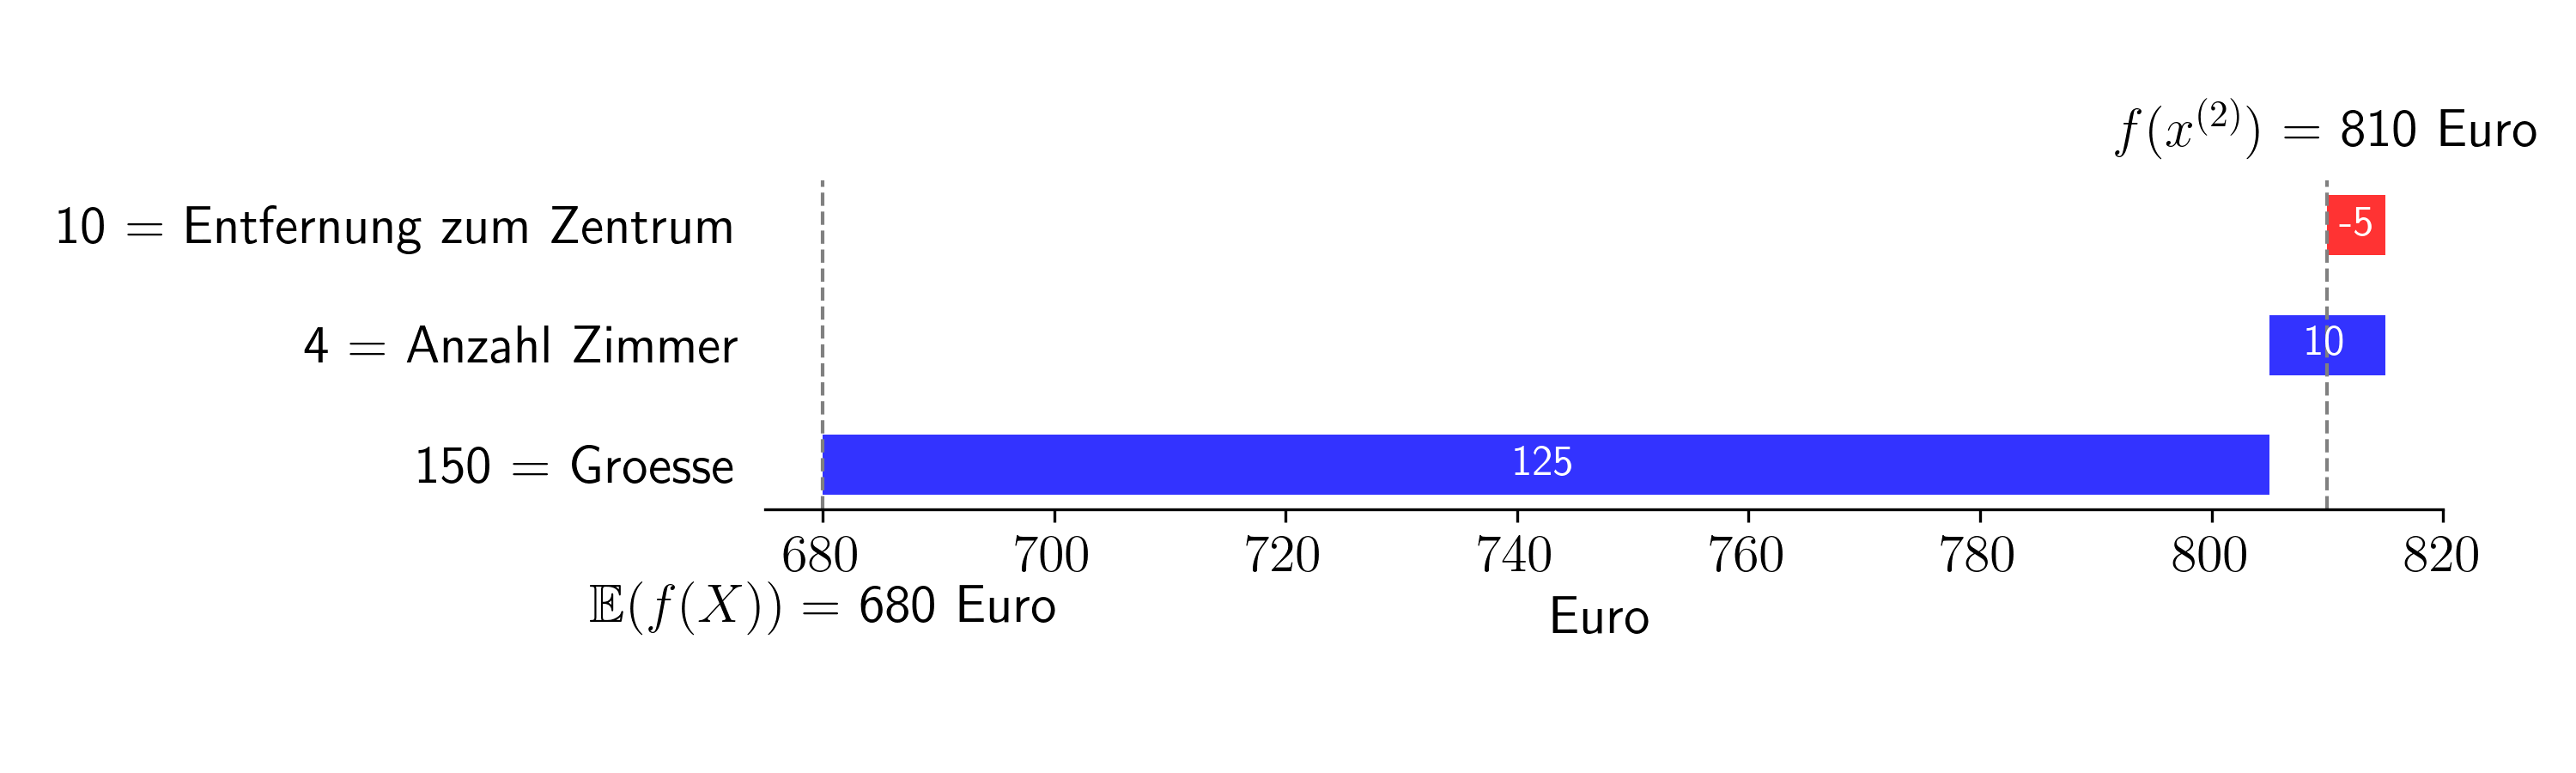
\includegraphics[width=1\textwidth]{../scripts/images/model-output-x2.png}
    Quelle: Eigene Darstellung, \ref{charts}.
    \label{pic:model-fx2}
\end{figure}


\section{Kontextualisierte axiomatische Grundlage der Shapley-Werte}

Die in Tabellen \ref{tab:shapley_marginal_features_x1} und \ref{tab:shapley_marginal_features_x2} präsentierten Ergebnisse bieten eine Grundlage, 
um die Konformität der SHAP-Werte mit den etablierten Axiomen der Shapley-Werte, wie sie im 
Kapitel \ref{sec:axiome-shapley} diskutiert wurden, zu beurteilen. Die Axiome der SHAP-Werte stellen 
eine adaptierte und kontextualisierte Anwendung dieser Prinzipien auf die Interpretation von 
Modellvorhersagen dar \cite[S. 16f]{Algaba2019HandbookOT}.


\paragraph{Effizienz}

Das Effizienzaxiom besagt, dass die Summe der SHAP-Werte aller Merkmals für eine gegebene Beobachtung $x^{(i)}$ 
gleich der Differenz zwischen der Modellvorhersage für diese Beobachtung $f(x^{(i)})$ 
und der durchschnittlichen Modellvorhersage $\mathbb{E}(f(X))$ sein muss:

\begin{align}
    \sum_{j=1}^{p}\varphi_j^{(i)}(\mathcal{N}, f) = f(x^{(i)}) - \mathbb{E}(f(X)),
    \label{eq:eff}
\end{align}

\cite[S. 221]{Molnar_2022}. Für die Beobachtung $x^{(1)}$ aus Kapitel \ref{sec:example} und den Berechnungen 
für $f(x^{(1)})$ (Gleichung \ref{eq:fx1}), sowie $\mathbb{E}(f(X))$ (Gleichung \ref{eq:efx}) ergibt sich:

\begin{align}
    \sum_{j=1}^{3}\varphi_j^{(1)}(\mathcal{N}, f) &=  -130 \\ \notag
    f(x^{(1)}) - \mathbb{E}(f(X)) &= 550 - 680 = -130,   
\end{align}

womit das Effizienzaxiom erfüllt ist. Die Differenz der Vohersage 
einer konkreten Beobachtung zur durchschnittlichen 
Modellvorhersage wird auf alle Merkmale verteilt.

\paragraph{Symmetrie}

Das Symmetrieaxiom fordert, dass zwei Merkmale $i$ und $j$, die 
in jeder Koalition denselben Beitrag leisten, auch denselben SHAP-Wert 
erhalten müssen. In dem hier betrachteten Fall der Immobilienpreisprognose 
würde dies bedeuten, dass wenn zwei Merkmale, beispielsweise die Größe einer 
Wohnung und die Anzahl der Zimmer, immer den gleichen Einfluss auf den Preis hätten, 
unabhängig von der Kombination anderer Merkmale, ihre SHAP-Werte identisch 
sein müssen:

\begin{equation}
    v(\mathcal{S} \cup \{i\}) = v(\mathcal{S} \cup \{j\}), \; \forall\, \mathcal{S} \subseteq \mathcal{N} \setminus \{i, j\} \Rightarrow \varphi_i (\mathcal{N}, v) = \varphi_j (\mathcal{N}, v),
\end{equation}

\cite[S. 221]{Molnar_2022}. Dies wird durch die Tabellen \ref{tab:shapley_marginal_features_x1} und \ref{tab:shapley_marginal_features_x2} 
nicht illustriert, da jedes Merkmal einen unterschiedlichen Beitrag liefert, 
was die Anwendung dieses Axioms in diesem speziellen Fall ausschließt.

\paragraph{Null-Spieler-Eigenschaft (Dummy-Spieler-Eigenschaft)}

Ein Merkmal $i$, das keinen Einfluss auf die Modellvorhersage hat, erhält gemäß der 
Null-Spieler-Eigenschaft einen SHAP-Wert von Null. 
Im Kontext des Beispiels würde ein Merkmal, das keine Veränderung in der Vorhersage 
bewirkt, unabhängig von den anderen Merkmalen, einen SHAP-Wert von Null erhalten:

\begin{equation}
    v(\mathcal{S} \cup \{i\}) =  v(\mathcal{S}), \; \forall\, \mathcal{S} \subseteq \mathcal{N} \setminus \{i\} \Rightarrow \varphi_i (\mathcal{N}, v) = 0,
\end{equation}

\cite[S. 222]{Molnar_2022}. In der fiktiven Datenlage der Tabellen \ref{tab:shapley_marginal_features_x1} und \ref{tab:shapley_marginal_features_x2} hat jedes Merkmal 
einen gewissen Einfluss, sodass die Null-Spieler-Eigenschaft hier nicht beobachtet werden kann.

\paragraph{Additivität}

Das Additivitätsaxiom ist ein zentrales Konzept, das die Konsistenz von Shapley-Werten 
über die Zusammensetzung von Spielen hinweg beschreibt. Es garantiert, 
dass für zwei separate Spiele oder Modelle \(v\) und \(w\), die Summe der SHAP-Werte eines 
Merkmals über beide Spiele seinem SHAP-Wert im kombinierten Spiel entspricht:

\begin{equation}
    \varphi_i(\mathcal{N}, v + w) = \varphi_i (\mathcal{N}, v) + \varphi_i (\mathcal{N}, w).
\end{equation}

In Machine Learning-Modellen wie dem Random Forest, besonders bei Ensemble-Modellen, 
ist die Additivität relevant. Ein Random Forest besteht aus unabhängigen Entscheidungsbäumen, 
die zusammenarbeiten, um Vorhersagen zu treffen. Die SHAP-Werte der einzelnen Bäume 
können als additive Beiträge betrachtet werden, die den Gesamteinfluss eines Merkmals 
auf die Modellvorhersage zusammenfassen. \cite[S. 32]{Molnar_2023}.

\chapter{Komplexitätsbewältigung bei der Berechnung von SHAP-Werten}
\label{sec:estimators}

Die direkte Berechnung von SHAP-Werten kann bei Modellen mit einer 
großen Anzahl an Merkmalen rechnerisch anspruchsvoll sein. Im Kontext linearer Modelle, 
wie dem in dieser Arbeit verwendeten Immobilienpreis-Beispiel, 
ist die vollständige Ermittlung aller möglichen Kombinationen von Merkmalen und deren 
Beiträgen jedoch nicht notwendig. 

In einem linearen Modell sind die Beiträge der einzelnen Merkmale zur Vorhersage additiv 
und unabhängig voneinander. Dies ermöglicht eine direkte Ableitung der Beiträge 
jedes Merkmals aus den Modellkoeffizienten. Aufgrund dieser Eigenschaft 
liefert jedes Merkmal einen konstanten marginalen Beitrag, 
unabhängig von der Zusammensetzung der restlichen Koalition von Merkmalen. 
Theoretisch könnte daher für jedes Merkmal nur eine Koalition berechnet werden, 
um den SHAP-Wert zu bestimmen \cite[S. 38]{Molnar_2023}. Dies bestätigen die
Tabellen \ref{tab:shapley_marginal_features_x1} und \ref{tab:shapley_marginal_features_x2}
und die daraus ersichtlichen marginalen Beiträge, die über die jeweiligen Merkmale
unabhängig der ihnen beigetretenen Koalition konstant sind. So ist der marginale Beitrag für Merkmal $x_1^{(1)}$
zu allen möglichen Koalitionen stets $-125$.

Die Herausforderung bei der Berechnung von SHAP-Werten in realen Szenarien erwächst aus 
zwei zentralen Problembereichen: der Anzahl der Merkmale und der Notwendigkeit, 
über diese Merkmale zu integrieren. 

Die Anzahl möglicher Koalitionen von Merkmalen wächst exponentiell mit \( 2^p \) an, 
was bei einer großen Anzahl von Merkmalen \( p \) schnell zu einer nicht handhabbaren Berechnungskomplexität führt. 
Hinzu kommt die Schwierigkeit, dass für eine exakte Berechnung der SHAP-Werte eine Integration 
über die Merkmalsverteilungen erforderlich ist, was jedoch voraussetzt, dass die Verteilung der Merkmale bekannt ist. 
In der Praxis verfügt man meist nur über eine Stichprobe der Daten, ohne genaue Kenntnis der zugrundeliegenden Verteilungen \cite[S. 33]{Molnar_2023}.

Um diesen Herausforderungen zu begegnen, wird in diesem Kapitel die Anwendung von Monte Carlo Integration 
zur Schätzung von SHAP-Werten diskutiert. Diese Methoden ermöglichen es, durch Zufallsstichproben aus den vorhandenen Daten 
eine Approximation der Verteilungen zu erstellen und dadurch die notwendigen Integrationen näherungsweise auszuführen \cite[S. 34]{Molnar_2023}. 
Darüber hinaus werden Ansätze zur Stichprobenbildung von Koalitionen vorgestellt, die es erlauben, 
die rechnerische Last zu reduzieren, indem nicht alle Koalitionen betrachtet, sondern repräsentative Stichproben gezogen werden. 

\section{Approximation der marginalen Beiträge mittels Monte Carlo Integration}

Statt das Integral über eine unbekannte Verteilung zu berechnen, wie in Gleichung \ref{eq:shap-value-func},
nähert die Monte Carlo Integration dieses Integral durch den Durchschnitt einer großen Anzahl zufällig 
ausgewählter Beobachtungen aus dem Eingaberaum an \cite[S. 34]{Molnar_2023}. Die Monte Carlo Integration kann als ein erwartungstreuer Schätzer 
betrachtet werden, wenn die Anzahl der Zufallsstichproben $n$ hinreichend groß ist. Dies bedeutet, dass mit zunehmendem $n$ die Schätzung des Integrals 
immer genauer wird und gegen den wahren Wert des Integrals konvergiert. Dies basiert auf dem Gesetz der großen Zahlen, 
das besagt, dass der Durchschnitt einer großen Anzahl unabhängiger und identisch verteilter Zufallsvariablen gegen den Erwartungswert der Verteilung konvergiert \cite[S. 83]{Robert_Casella_2004}. 

Die Zufallsvariable $X_{C}^{(k)}$, die Merkmale die nicht in der Koalition $\mathcal{S}$ enthalten sind, 
entfällt und wird durch konkrete Beobachtungen $x_{C}^{(k)}$ aus der Datenbasis ersetzt, 
was eine wünschenswerte Vereinfachung darstellt. Das Integral $\int$ wird dadurch zur Summe $\sum$ und die Verteilung $\mathbb{P}$ wird durch eine große Anzahl zufällig 
ausgewählter Beobachtungen ersetzt und das Ergebnis anschließend über alle ausgewählten Beobachtungen $n$ gemittelt. 
$\hat{v}_{x^{(i)}, f}(\mathcal{S})$ ist somit ein Schätzer für den Wert der Koalition $\mathcal{S}$ und definiert als: 

\begin{align}
    \label{eq:monte-value}
    \hat{v}_{x^{(i)},f}(\mathcal{S}) = \frac{1}{n} \sum_{k=1}^{n} \Big(f(x^{(i)}_{\mathcal{S}} \cup x^{(k)}_{C}) - f(x^{(k)}) \Big)
\end{align}

Analog zu Gleichung \ref{eq:shap-marginal-func} ist dann zusammen mit Gleichung \ref{eq:monte-value} der marginale Beitrag 
$\hat{\Delta}_{\mathcal{S}, j}$ von Merkmal $j$ zur Koalition $\mathcal{S}$ gegeben als: 

\begin{align}
    \label{eq:monte-mar}
    \hat{\Delta}_{\mathcal{S}, j} &= \hat{v}_{x^{(i)},f}(\mathcal{S} \cup \{j\}) - \hat{v}_{x^{(i)},f}(\mathcal{S}) \\ \notag
        &= \frac{1}{n} \sum_{k=1}^{n} \Big(f(x^{(i)}_{\mathcal{S} \cup \{j\}} \cup x^{(k)}_{C \setminus \{j\}}) - f(x^{(i)}_{\mathcal{S}} \cup x^{(k)}_{C}) \Big)
\end{align}

und die SHAP-Werte $\hat{\varphi}_{j}^{(i)}$ über alle möglichen Koalitionen analog zu Gleichung \ref{eq:shap-eq}:

\begin{align}
    \label{eq:monte-shap-eq}
    \hat{\varphi}^{(i)}_{j} (\mathcal{N}, f) &= \sum_{\mathcal{S} \subseteq \mathcal{N} \setminus \{j\}} \frac{|\mathcal{S}|! \cdot (p - 1 - |\mathcal{S}|)!}{p!}\hat{\Delta}_{\mathcal{S}, j},
\end{align}

\cite[S.36]{Molnar_2023}.

\section{Schätzung von Koalitionen}

Obwohl die Monte Carlo Integration aus Gleichung \ref{eq:monte-shap-eq} eine praktische Methode zur Approximation der benötigten marginalen Beiträge in der 
SHAP-Wertberechnung bietet, bleibt die Herausforderung, alle möglichen Koalitionen der Merkmals zu evaluieren. 
Die Anzahl der Koalitionen wächst exponentiell mit der Anzahl der Merkmals. Daher sind Ansätze gefragt, die eine effiziente Schätzung der SHAP-Werte erlauben, 
ohne jede mögliche Koalition explizit zu berücksichtigen.

Insbesondere für lineare Modelle ohne Interaktionsterme wurde in Kpaitel \ref{sec:estimators} bereits gezeigt,
dass die Berechnung einer einzigen Koalition für jedes Merkmal ausreichend ist \cite[S. 38]{Molnar_2023}.
In einem solchen Modell wird angenommen, dass die Beziehung zwischen den unabhängigen 
Variablen und der abhängigen Variable additiv ist, das heißt, es gibt keine Terme im Modell, 
die das Produkt von zwei oder mehr unabhängigen Variablen enthalten, um mögliche Interaktionseffekte 
zwischen ihnen zu repräsentieren.

Neben dem Linearen SHAP Estimator in Kapitel \ref{subsec:linear-shap-estimator} wird die Schätzung durch Permutationen in Kapitel 
\ref{subsec:permutation} diskutirert. Anstelle der Iteration über alle Koallitionen, werden repräsentative Stichproben zur Berechnung
herangezogen. 

Beide Verfahren bieten Strategien zur Reduzierung der Berechnungskomplexität, 
indem sie Annahmen über die Eigenschaften des Modells und der Daten treffen. 
Weitere Ansätze werden in Kapitel \ref{sec:shap-package} angesprochen.


\subsection{Linearer SHAP Estimator für lineare Modelle}
\label{subsec:linear-shap-estimator}

Für lineare Modelle bietet der lineare SHAP Estimator eine direkte und effiziente 
Methode zur Berechnung der SHAP-Werte. Diese Methode beruht auf der Annahme 
der Unabhängigkeit der Eingabemerkmale. Unter dieser Voraussetzung können 
die SHAP-Werte direkt aus den Gewichtungskoeffizienten des linearen Modells 
abgeleitet werden.

Ein lineares Modell wird typischerweise in der Form 
\( f(x) = \sum_{j=1}^{p} \beta_j x_j + b \) ausgedrückt, wobei \( \beta_j \) der 
Gewichtungskoeffizient für das Merkmal \( j \) ist und \( b \) den 
Achsenabschnitt (Bias) darstellt. Der lineare SHAP Estimator nutzt 
diese Koeffizienten, um die Beiträge jedes Merkmals zur Modellvorhersage 
zu bestimmen. Der SHAP-Wert für ein Merkmal \( j \) wird dann definiert als:

\begin{align}
    \varphi_j^{(i)}(f, x) = \beta_j (x_j^{(i)} - \mathbb{E}[X_j]),
\end{align}

wobei \( \mathbb{E}[X_j] \) der Erwartungswert des Merkmals \( j \) über den 
Datensatz ist. Der SHAP-Wert für den Achsenabschnitt (Bias) ist gleich 
dem Achsenabschnitt des Modells: \( \varphi_0(f, x) = b \) \cite[S. 6]{NIPS2017_8a20a862}.

Aufgrund der Unabhängigkeit der Eingabemerkmale, kann das arithmetische Mittel aus Kapitel 
\ref{sec:example} Gleichung \ref{eq:e} als erwartungstreuer Schätzer für den Erwartungswert verwendet werden:

\begin{align}
    \varphi_j^{(i)}(f, x) = \beta_j \Big(x_j^{(i)} - \frac{1}{n} \sum_{k=1}^{n} (x_j^{(k)})\Big),
\end{align}

Das Effizienzaxiom aus Gleichung \ref{eq:eff} is erfüllt:

\begin{align}
    \sum_{j=1}^p \varphi_j^{(i)}(f, x) &= \sum_{j=1}^p  \Big( \beta_j x_j^{(i)} - \mathbb{E}[\beta_j X_j]\Big) \\ \notag
                                    &= \beta_0 + \sum_{j=1}^p \beta_j x_j^{(i)} - ( \beta_0 + \sum_{j=1}^p \mathbb{E}[\beta_j X_j]) \\ \notag
                                    &= f(x) - \mathbb{E}[f(X)],
\end{align}                 

\cite[S. 48]{Molnar_2023}.

Diese Berechnung der SHAP-Werte basiert auf der Idee, dass die Änderung 
des Modelloutputs, die durch das Abweichen eines Merkmals von seinem 
Erwartungswert entsteht, direkt durch den entsprechenden Gewichtungskoeffizienten 
des linearen Modells beschrieben werden kann. Dieser Ansatz ermöglicht eine 
schnelle und genaue Berechnung der SHAP-Werte für lineare Modelle und ist 
besonders nützlich, um die Auswirkungen einzelner Merkmals in einem solchen 
Modell zu interpretieren. 

\subsection{Schätzung durch Permutationen}
\label{subsec:permutation}

Der Einsatz von Permutationen zur Schätzung von SHAP-Werten bietet eine 
praktikable Alternative zur vollständigen Auswertung aller Merkmalskoalitionen. 
Dieses Verfahren ist insbesondere in Szenarien mit einer hohen Anzahl von Merkmalen von Vorteil, 
da es die Berechnungslast reduziert, ohne die Genauigkeit der Schätzung wesentlich zu beeinträchtigen. 
Im Folgenden wird die Methode anhand eines Beispiels illustriert und die Anwendung im Kontext des in 
Kapitel \ref{sec:example} eingeführten linearen Modells beschrieben.

In einem ersten Schritt wird eine zufällige $k$-te Permutation der Merkmale $o(k)$ gewählt.
Beispielsweise könnte $o(k) = (x_2, x_3, x_1)$ eine solche Permutation darstellen.
Wird das Merkmal $j$, für das der SHAP-Wert berechnet werden soll, als das dritte Merkmal $j=3$ angenommen, 
ergibt sich der marginale Beitrag $\hat{\Delta}_{o(k), j}$ analog zu Gleichung \ref{eq:monte-mar} 
aus der Differenz der Koalitionen mit und ohne dem betrachteten Merkmal:

\begin{align}
    \hat{\Delta}_{o(k), j} = \hat{v}(\{x_2, x_3\}) - \hat{v}(\{x_2\})
\end{align}

Dieser Prozess wird für eine Anzahl von $m$ Permutationen durchgeführt. Die Wahl von $m$,
die kleiner als die Gesamtzahl der Merkmale sein kann, hängt von der gewünschten Approximationsgenauigkeit
ab. Eine größere Anzahl von Permutationen $m$ führt zu einer präziseren Annäherung an den tatsächlichen SHAP-Wert.

Die geschätzten marginalen Beiträge $\hat{\Delta}_{o(k), j}$ werden dann über die $m$ Permutationen analog zu Gleichung
\ref{eq:monte-shap-eq} gemittelt:

\begin{align}
    \label{eq:permu-shap-eq}
    \hat{\varphi}^{(i)}_{j} (\mathcal{N}, f) &= \frac{1}{m}\sum_{k=1}^{m}\hat{\Delta}_{o(k), j},
\end{align}

Durch diese Methodik wird der Berechnungsaufwand bei der Ermittlung von SHAP-Werten 
signifikant verringert, was besonders bei Modellen mit einer großen Anzahl von Merkmalen von 
Bedeutung ist. Der hier vorgestellte Ansatz ermöglicht es, mit einer begrenzten Anzahl von 
Permutationen eine aussagekräftige Schätzung der SHAP-Werte zu erhalten \cite[S. 39]{Molnar_2023}.

Zusätzlich zur Mittelung der geschätzten marginalen Beiträge bietet die Methode der Permutationen 
die Möglichkeit, die Effekte von Vorwärts- und Rückwärtspropagation zu untersuchen, 
indem die Reihenfolge der Merkmale sowohl in ihrer ursprünglichen als auch in umgekehrter 
Abfolge betrachtet wird. Für eine detaillierte Darstellung dieser Technik und ihrer 
Auswirkungen auf die SHAP-Wertberechnung sei auf die weiterführende Literatur verwiesen \cite[S. 39f]{Molnar_2023}.


